\documentclass{beamer}

\usepackage{ae,lmodern} 
\usepackage[french]{babel}
\usepackage[utf8]{inputenc}
\usepackage[T1]{fontenc}
\usepackage{geometry}
\usepackage{multicol}
\usepackage{graphicx}
\usepackage{enumitem}
\usepackage{fixltx2e}
\usepackage{amsmath}
\usepackage{nccmath}
\usepackage{amssymb}
\usepackage{dsfont}
\usepackage{stmaryrd}
\usepackage{mathtools}
\usepackage{scalerel}
\usepackage{bbold}
\usepackage{natbib}

\usetheme{Warsaw}
\setbeamertemplate{frame numbering}[fraction]
\setbeamertemplate{frametitle}[default][center] 


\author{SELVESTREL Alexandre, KAMARY Kaniav}
\title{Bayesian model choice via mixture estimation model : Poisson versus Geometric regression models}
\date{} 

\begin{document}
\setbeamertemplate{caption}[numbered]

\begin{frame}
\titlepage
\end{frame}

\begin{frame}
\tableofcontents
\end{frame}

\begin{frame}
\nocite{kamary2018testing}
\section{Introduction}
\nocite{kamary2018testing}
\begin{center}
\textbf{Problem of model selection in the bayesian framework}\\[10 pt]


  \begin{columns}
    \begin{column}{0.5\textwidth}
      \begin{figure}
        \centering
        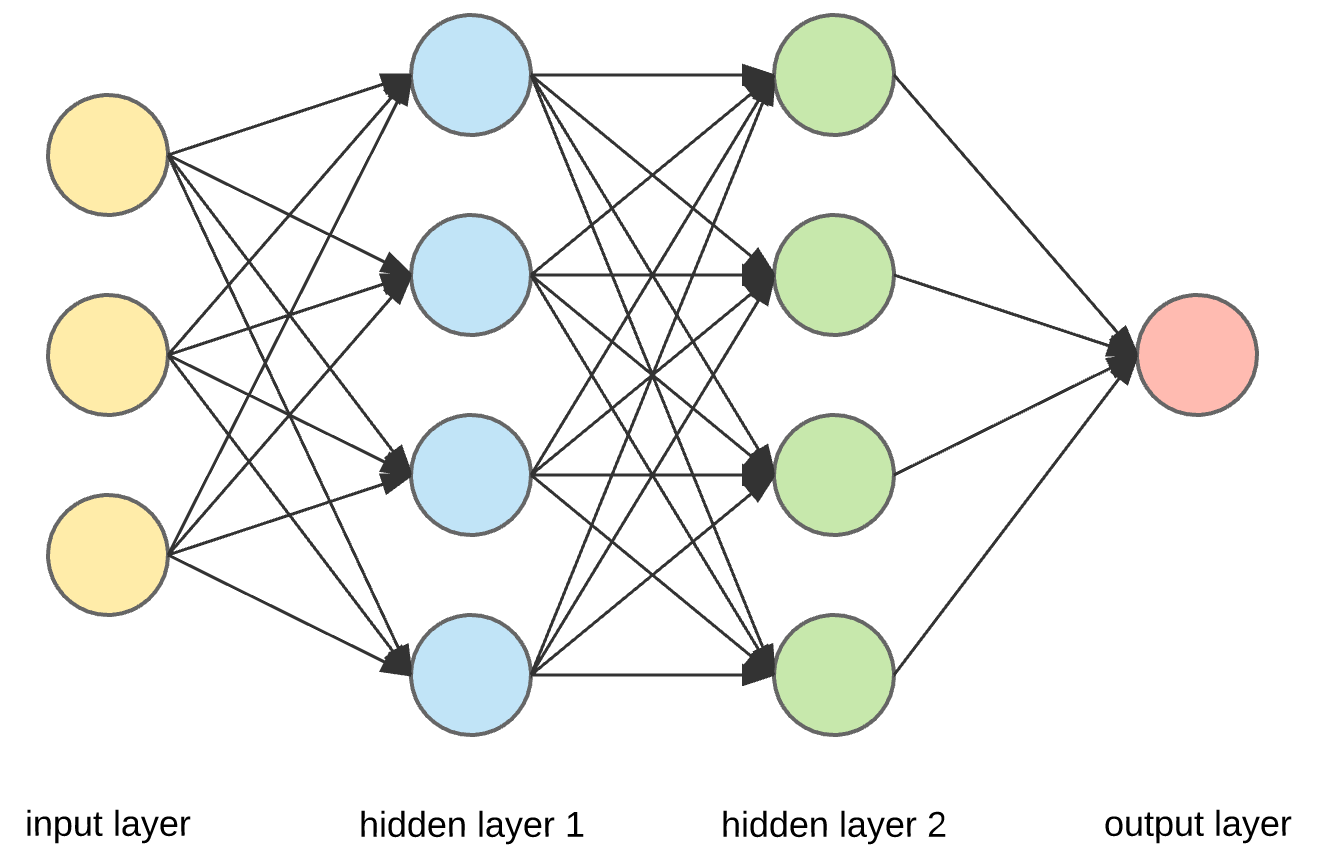
\includegraphics[width=\textwidth]{nn_1.png}
        \caption{A shallow neural network}
      \end{figure}
    \end{column}
    \begin{column}{0.5\textwidth}
      \begin{figure}
        \centering
        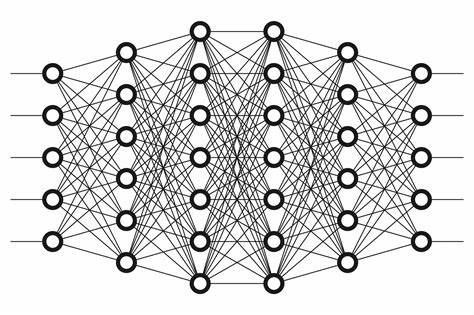
\includegraphics[width=\textwidth]{nn_2.jpeg}
        \caption{A deeper neural network}
      \end{figure}
    \end{column}
  \end{columns}
\end{center}


\end{frame}

\begin{frame}
\begin{center}
\textbf{Question of the activation function:} 
\end{center}

  \begin{columns}
    \begin{column}{0.25\textwidth}
      \begin{figure}
        \centering
        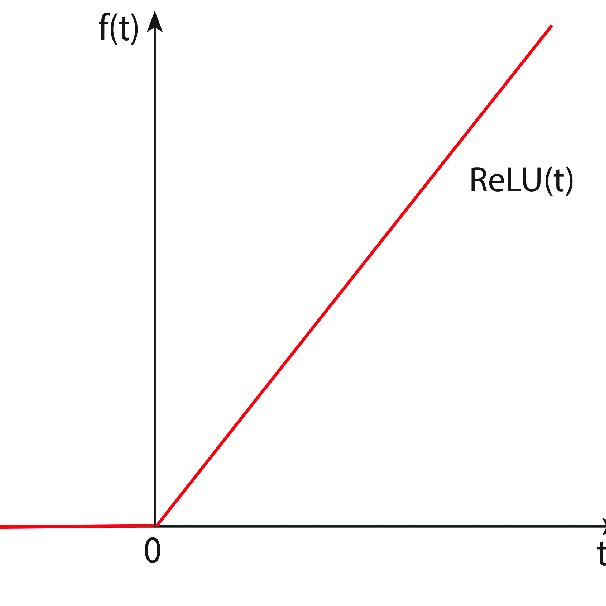
\includegraphics[width=\textwidth]{relu.jpg}
        \caption{ReLU function}
      \end{figure}
    \end{column}
    \begin{column}{0.33\textwidth}
      \begin{figure}
        \centering
        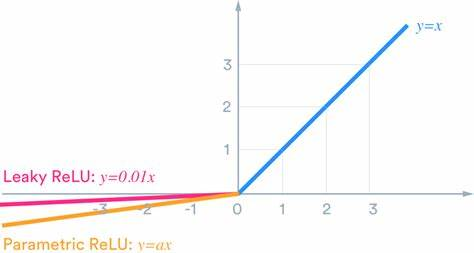
\includegraphics[width=\textwidth]{lrelu.jpeg}
        \caption{Leaky ReLU function}
      \end{figure}
    \end{column}
    \begin{column}{0.33\textwidth}
      \begin{figure}
        \centering
        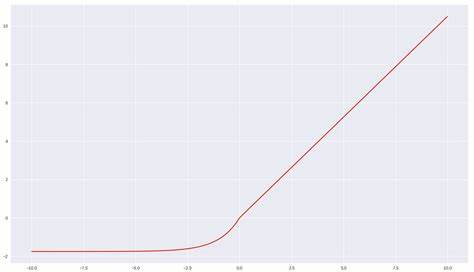
\includegraphics[width=\textwidth]{selu.jpeg}
        \caption{SeLU function}
      \end{figure}
    \end{column}
  \end{columns}
\end{frame}

\begin{frame}
\begin{center}
\textbf{Very high number of parameters (without regularisation)}
\end{center}
Example of resnet: \citep{he2015deep}

\begin{figure}[H]
\centering
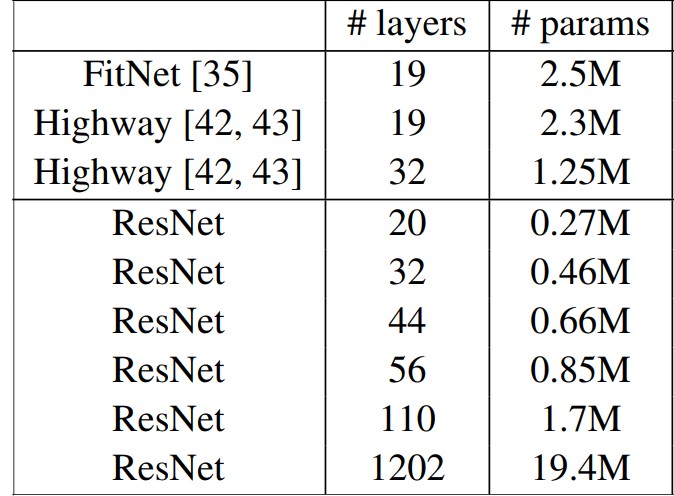
\includegraphics[scale=0.20]{high_param.png}
\caption{Number of parameters for different neural networks} 
\label{fig:1}
\end{figure}
\onslide<2->{
\begin{equation}
\text{AIC} = 2(\text{Card(param)} - \log(\hat{L}))
\end{equation}
VC dimension: maximal number of point such that there exists a generally positioned data point set of 
 that can be shattered by the model

}

\end{frame}

\begin{frame}
\begin{center}
\textbf{Need for Bayesian methods}\\[20 pt]
\end{center}
  \begin{itemize}
    \item[$\bullet$] Go further than a simple balance to strike between accuracy on the training data set and over-fitting\\[8 pt]
    \item[$\bullet$] More interpretability\\[8 pt]
    \item[$\bullet$] More understanding of our uncertainty
  \end{itemize}
\end{frame}

\begin{frame}
\section{Overview of bayesian methods for model selection}
\frametitle{Bayes Factor}

\begin{equation}
B_{01} = \displaystyle{\frac{\displaystyle{\frac{P(H_0|x)}{P(H_1|x)}}}{\displaystyle{\frac{P(H_0)}{P(H_1)}}}} = \displaystyle{\frac{P(H_0|x)P(H_1)}{P(H_1|x)P(H_0)}}
\end{equation}

Advantage: 
\begin{itemize}
\item[$\bullet$] Allows to clearly see the dependency on initial hypothesis (or to "eliminate" it partially...)
\item[$\bullet$] Shows the importance of new data
\end{itemize}

\onslide<2->{
Disadvantages:
\begin{itemize}
\item[$\bullet$] Just a description of the "evolution" of the probability
\item[$\bullet$] No penalization nor finegrained description of uncertainty
\end{itemize}
}
\end{frame}

\begin{frame}
\frametitle{Directly giving (hierarchical) probabilities to hypothesis}


\end{frame}


\begin{frame}
\bibliographystyle{plainnat} % Choose your bibliography style
\bibliography{references}
\end{frame}





















\end{document}